\documentclass[11pt]{article}

% Core packages (robust to minimal TeX installs)
\usepackage[margin=1in]{geometry}
\usepackage{graphicx}
\usepackage{booktabs}
\usepackage{amsmath,amssymb}
\usepackage{url}

% Optional enhancements (safe to comment out if your TeX install is minimal)
% \usepackage{hyperref}
% \usepackage{microtype}

% Matheus style file: try .sty first, then fallback to .tex
\IfFileExists{matheus-style.sty}{%
  \usepackage{matheus-style}%
}{%
  \IfFileExists{matheus-style.tex}{% matheus-style.tex
% reusable style file for all papers by matheus maldaner
% last updated: 2026-02-21
%
% usage: copy into paper directory, add \usepackage{matheus-style} to preamble
% this file layers on top of venue-specific .sty/.cls files

\ProvidesPackage{matheus-style}

% --- core packages (safe to load alongside most venue templates) ---
\RequirePackage{booktabs}          % professional tables (\toprule, \midrule, \bottomrule)
\RequirePackage{graphicx}          % \includegraphics
\RequirePackage{subcaption}        % subfigures with (a), (b), (c) labels
\RequirePackage{amsmath,amssymb}   % standard math environments
\RequirePackage{float}             % [H] placement option
\RequirePackage[most]{tcolorbox}   % algorithm boxes, callout boxes
\RequirePackage{enumitem}          % list customization (noitemsep, etc.)
\RequirePackage{xcolor}            % named colors
\RequirePackage{xspace}            % smart spacing after macros

% --- algorithm box (matches thesis style) ---
% clean horizontal-rule-only box for pseudocode
\newtcolorbox{algorithmbox}[1][]{
    enhanced,
    colback=white,
    colframe=black,
    boxrule=0pt,
    borderline north={0.8pt}{0pt}{black},
    borderline south={0.8pt}{0pt}{black},
    left=8pt,
    right=8pt,
    top=6pt,
    bottom=6pt,
    before skip=8pt,
    after skip=8pt,
    sharp corners,
    #1
}

% --- colorblind-safe palette (tol bright) ---
\definecolor{cblue}{HTML}{0072B2}
\definecolor{corange}{HTML}{D55E00}
\definecolor{cgreen}{HTML}{009E73}
\definecolor{cpink}{HTML}{CC79A7}
\definecolor{cyellow}{HTML}{F0E442}
\definecolor{csky}{HTML}{56B4E9}
\definecolor{cgray}{HTML}{999999}

% --- math shortcuts ---
\newcommand{\R}{\mathbb{R}}
\newcommand{\N}{\mathbb{N}}
\newcommand{\Z}{\mathbb{Z}}
\newcommand{\E}{\mathbb{E}}
\DeclareMathOperator{\argmax}{arg,max}
\DeclareMathOperator{\argmin}{arg,min}
\DeclareMathOperator{\softmax}{softmax}
\DeclareMathOperator{\sigmoid}{\sigma}

% --- text shortcuts ---
\newcommand{\ie}{i.e.,\xspace}
\newcommand{\eg}{e.g.,\xspace}
\newcommand{\cf}{cf.\xspace}
\newcommand{\etal}{et al.\xspace}
\newcommand{\wrt}{w.r.t.\xspace}

% --- typography ---
\clubpenalty=10000   % no orphans
\widowpenalty=10000  % no widows

% --- float spacing ---
\setlength{\floatsep}{10pt}
\setlength{\textfloatsep}{12pt}
\setlength{\intextsep}{8pt}}{}%
}

\title{Crisis Lens: The Overlooked Crisis Index for Humanitarian Funding Gaps}
\author{
Andrew Vu \\ University of Florida
\and Matheus Maldaner \\ University of Florida
\and Raami Abichou \\ University of Florida
\and Jeremy Hur \\ Georgia Institute of Technology
}
\date{February 2026}

\begin{document}
\maketitle

\begin{abstract}
Humanitarian funding does not align with need, and existing public dashboards do not make the mismatch easy to quantify or act on. We present Crisis Lens, a hackathon system that computes an Overlooked Crisis Index (OCI) and pairs it with an interactive map, cluster level drilldowns, efficiency outlier detection, and a project recommender. The OCI combines people in need normalized by population, a derived severity proxy, funding gap, and a media attention penalty. Using UN HNO, FTS, population, and CBPF data from 2024 to 2026, we score 24 crisis contexts and analyze 8,091 projects. In the latest year, the mean funding gap across tracked crises is 0.917, and the most overlooked contexts are South Sudan (OCI 1.000), Syria (0.982), Yemen (0.915), Sudan (0.851), and Haiti (0.686). At the project level, 265 high efficiency benchmarks show a median beneficiary to budget ratio 15.6x the median of the remaining projects. We also identify 12 crises with increasing funding gaps and above median OCI scores, signaling worsening neglect. A Databricks notebook reproduces the full pipeline and visualizations for audit and reuse.
\end{abstract}

\section{Introduction}
Humanitarian response faces a persistent allocation problem, resources do not track need with enough precision to guide timely action. We address this gap by defining a single index that merges severity, funding coverage, and media attention, then pairing it with tools that operate at the levels where decisions are made. Crisis Lens is a hackathon system built for the Databricks x United Nations Geo Insight Challenge, and it provides an end to end workflow from data ingestion to actionable recommendations.

This paper makes three contributions. First, we define the Overlooked Crisis Index (OCI), a normalized score that captures how underfunded and underexposed a crisis is relative to its population. Second, we integrate five UN aligned data sources into a reproducible pipeline that produces country year scores, cluster level gaps, and project level efficiency signals. Third, we deliver an interactive product with a global map, drilldowns, an outlier finder, a recommender powered by vector search, and a funding trend forecast. Together these pieces align with the judging rubric for impact, scope, and technical depth.

The rest of the paper follows the structure used in the judging rubric, it first defines the OCI and data sources, then describes the system, then reports results, and ends with limitations and implications.

\section{Measuring Overlooked Crises}
\subsection{Data Sources}
We integrate public UN datasets that cover needs, funding, population, and project level allocations. Humanitarian Needs Overview (HNO) provides people in need, Global Requirements and Funding (FTS) provides requirements and funding received, COD PS population data enables normalization, and CBPF data provides project level budgets and beneficiaries. A media attention proxy from Google Trends adds a weak signal for public visibility when available. Table \ref{tab:data_summary} summarizes coverage.

\subsection{OCI Definition}
OCI is defined for each country year and normalized to a 0 to 1 range across all crises. Let $P$ be people in need, $N$ be population, $G$ be funding gap, $S$ be severity, and $M$ be a media neglect score. We compute
\begin{equation}
OCI = \left(\frac{P}{N}\right) \cdot \left(\frac{S}{5}\right) \cdot G \cdot \left(1 + 0.2 M\right)
\end{equation}
and min max normalize the result. Funding gap is $G = 1 - \frac{\text{funding}}{\text{requirements}}$ and is clipped to the 0 to 1 range. Because numeric OCHA severity is not available in the HNO files, we derive $S$ by placing the $P/N$ ratio into quintiles that map to the 1 to 5 scale. This proxy is a limitation, and we discuss it in Section \ref{sec:discussion}.

\subsection{Media Attention Proxy}
Media attention is estimated by Google Trends search interest for queries of the form ``[country] crisis'' over the past 12 months. When live lookup fails, we fall back to a static baseline derived from a January 2025 snapshot. We invert normalized interest so higher $M$ means lower attention and higher neglect.

\section{System and Implementation}
The pipeline is written in Python and runs in a Databricks notebook or locally. It downloads raw data, cleans and harmonizes columns, computes OCI, and saves processed CSVs for the Streamlit app. The app contains five pages: a global map, a crisis drilldown with cluster funding gaps, an efficiency outlier view, a project recommender, and a funding forecast.

Project level recommendations use cosine similarity over a feature vector that includes cluster type, organization type, log budget, and log beneficiaries. We use Actian VectorAI DB for vector search when available, with a fallback to scikit learn cosine similarity to ensure reproducibility. This satisfies the vector database challenge requirements without coupling the system to one backend.

\begin{figure}[t]
\centering
\IfFileExists{figures/databricks_notebook.png}{
  \includegraphics[width=\columnwidth]{figures/databricks_notebook.png}
}{
  \fbox{\parbox[c][2.0in][c]{0.9\columnwidth}{\centering Databricks notebook screenshot placeholder}}
}
\caption{Databricks notebook used to reproduce the data pipeline and visual outputs.}
\label{fig:databricks}
\end{figure}

\section{Results}
\subsection{Global Ranking of Overlooked Crises}
Figure \ref{fig:oci_map} shows the global OCI map for 2026, which highlights severe mismatches between needs and funding. Table \ref{tab:top5} lists the five highest OCI scores in 2026. The average funding gap across tracked crises in 2026 is 0.917, and the median is 0.923, indicating that many response plans remain far below requirements.

\begin{figure}[t]
\centering
\IfFileExists{figures/oci_map.pdf}{
  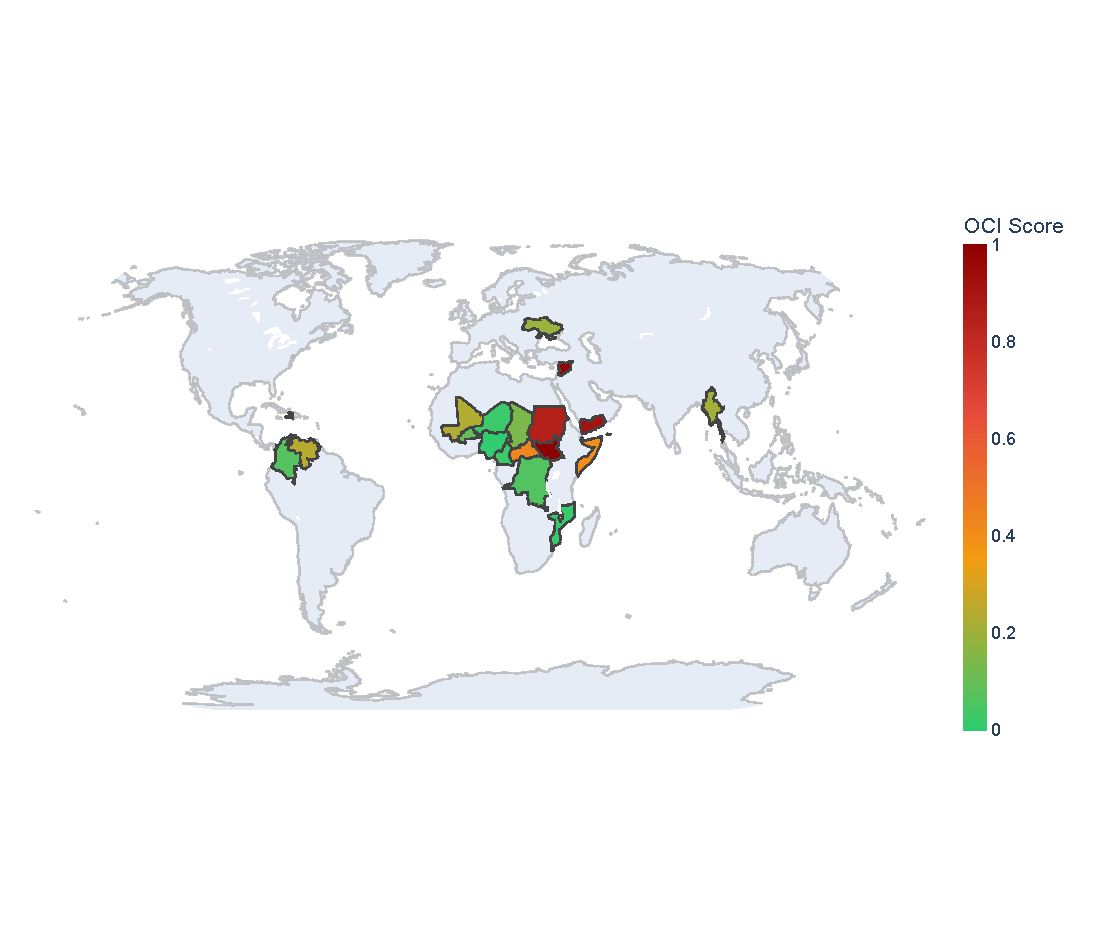
\includegraphics[width=\columnwidth]{figures/oci_map.pdf}
}{
  \fbox{\parbox[c][2.2in][c]{0.9\columnwidth}{\centering OCI map figure placeholder}}
}
\caption{Global Overlooked Crisis Index map for 2026. Higher values indicate more overlooked crises.}
\label{fig:oci_map}
\end{figure}

\begin{table}[t]
\centering
\caption{Data coverage used in Crisis Lens.}
\label{tab:data_summary}
\begin{tabular}{lrrl}
\toprule
Dataset & Rows & Countries & Years \\
\midrule
OCI scores (HNO + FTS + population) & 65 & 24 & 2024 to 2026 \\
FTS global funding & 1,069 & 105 & 2000 to 2026 \\
CBPF projects & 8,091 & 22 & 2020 to 2026 \\
Media attention scores & 24 & 24 & 2025 baseline \\
\bottomrule
\end{tabular}
\end{table}

\begin{table}[t]
\centering
\caption{Top five OCI scores for 2026. Funding gap is shown as a percent of unmet requirements.}
\label{tab:top5}
\begin{tabular}{lrrr}
\toprule
Country & OCI & Funding gap (\%) & People in need (M) \\
\midrule
South Sudan & 1.000 & 89.5 & 9.9 \\
Syria & 0.982 & 94.9 & 16.5 \\
Yemen & 0.915 & 93.0 & 23.1 \\
Sudan & 0.851 & 87.0 & 33.7 \\
Haiti & 0.686 & 96.3 & 6.4 \\
\bottomrule
\end{tabular}
\end{table}

\subsection{Cluster Level Funding Gaps}
Cluster funding gaps reveal which operational areas are most under resourced. For South Sudan in 2026, the largest gaps are Camp Coordination and Camp Management at 100.0\%, Logistics at 99.3\%, and Shelter and Non Food Items at 98.1\%. Figure \ref{fig:cluster_gap} visualizes these gaps, which align with field reports of access constraints and displacement.

\begin{figure}[t]
\centering
\IfFileExists{figures/cluster_gap_ssd_2026.pdf}{
  
\includegraphics[width=\columnwidth]{figures/cluster_gap_ssd_2026.pdf}
}{
  \fbox{\parbox[c][2.0in][c]{0.9\columnwidth}{\centering Cluster funding gap figure placeholder}}
}
\caption{Cluster funding gaps for South Sudan, 2026.}
\label{fig:cluster_gap}
\end{figure}

\subsection{Efficiency Outliers and Benchmark Projects}
At the project level, we compute beneficiary to budget ratios and flag outliers within each cluster and year using log scaled z scores. We identify 265 high efficiency benchmark projects out of 8,091 total projects. The median efficiency ratio of benchmarks is 0.469 beneficiaries per dollar, compared to 0.030 for the remaining projects, a 15.6x difference. Figure \ref{fig:outlier_scatter} shows the distribution of projects and highlights benchmarks. This gap provides a shortlist for cross context benchmarking, which the recommender surfaces through vector similarity.

\begin{figure}[t]
\centering
\IfFileExists{figures/outlier_scatter.pdf}{
  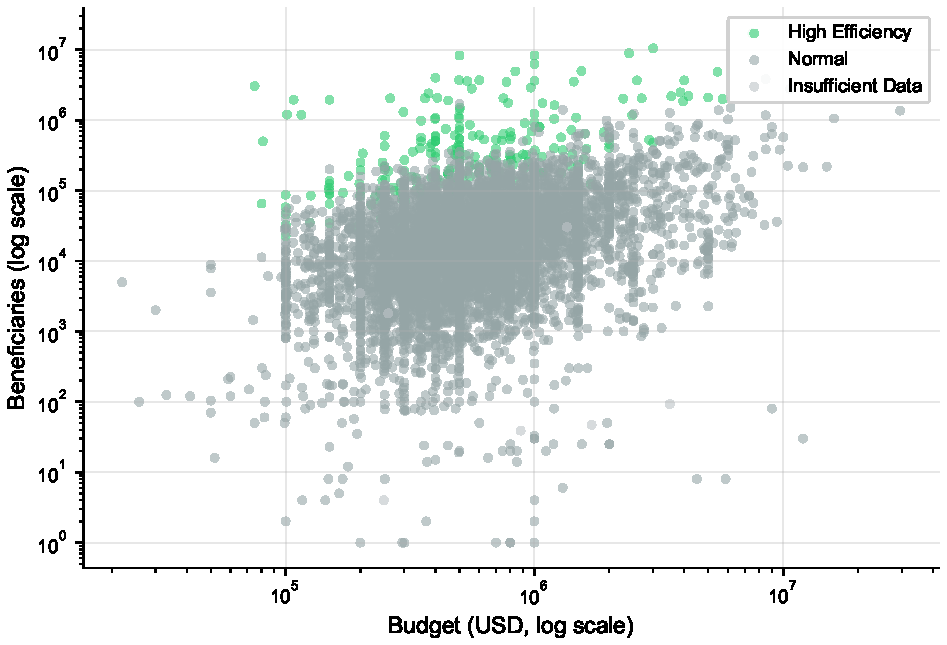
\includegraphics[width=\columnwidth]{figures/outlier_scatter.pdf}
}{
  \fbox{\parbox[c][2.2in][c]{0.9\columnwidth}{\centering Outlier scatter figure placeholder}}
}
\caption{Project budget vs. beneficiaries, highlighting high efficiency benchmarks.}
\label{fig:outlier_scatter}
\end{figure}

\subsection{Funding Trajectory Forecasts}
We fit linear trends to funding gap time series for each country with at least two years of data and project gaps to 2027. Twelve crises have positive funding gap slopes and above median OCI scores, indicating worsening neglect under current trends. The largest positive slopes occur in Ukraine (0.318 per year), South Sudan (0.306), and Central African Republic (0.297). Figure \ref{fig:forecast_trend} shows an example forecast for South Sudan. We treat these values as early warning signals rather than predictions, given the short time window and the potential for abrupt shocks.

\begin{figure}[t]
\centering
\IfFileExists{figures/forecast_trend_ssd.pdf}{
  
\includegraphics[width=\columnwidth]{figures/forecast_trend_ssd.pdf}
}{
  \fbox{\parbox[c][2.0in][c]{0.9\columnwidth}{\centering Forecast trend figure placeholder}}
}
\caption{Funding gap trend and 2027 projection for South Sudan.}
\label{fig:forecast_trend}
\end{figure}

\section{Discussion}
\label{sec:discussion}
This work aligns with UN data standards and builds on established reporting streams from HNO, FTS, and CBPF. The primary limitation is the lack of numeric OCHA severity in the public HNO files, which we approximate using $P/N$ quantiles. This proxy captures scale of need but does not model intensity of harm or conflict dynamics, which may reduce sensitivity in some contexts. Media attention is also a weak proxy, and it can be biased by news cycles, language, and search behavior.

Cluster inference for CBPF projects is keyword based, which can misclassify ambiguous titles. We mitigate this by using outliers only as candidate benchmarks rather than definitive judgments. Finally, linear trend forecasts are only descriptive, they should be treated as risk flags and paired with qualitative context from field teams.

Despite these limits, Crisis Lens demonstrates that public data can support a repeatable, actionable view of humanitarian neglect. The system surfaces clear prioritization cues that align with the Databricks x UN challenge goals and supports decision making at the cluster and project levels.

\section{Conclusion}
Crisis Lens provides a measurable definition of overlooked crises and a pipeline that translates disparate UN datasets into ranked priorities and operational insights. The OCI ranking highlights crises where funding gaps and population adjusted need converge, and the project level analysis highlights benchmarks that can inform more effective allocation. Our results show that severe underfunding persists across most tracked crises in 2026, and the system provides a direct path from global ranking to actionable project recommendations. The approach is lightweight enough for hackathon deployment while remaining transparent and reproducible.

\section*{Reproducibility Statement}
All data sources are public and listed in Table \ref{tab:data_summary}. The full pipeline is implemented in Python and runs either locally or in Databricks. We provide a Databricks notebook that downloads the data, reproduces the OCI computation, and generates the figures used in this paper. The Streamlit app reads processed CSVs from the pipeline, and all intermediate outputs are stored in a versioned data directory.

\begin{thebibliography}{9}
\bibitem{hno}
Humanitarian Needs Overview (HNO) data. \url{https://data.humdata.org/dataset/global-hpc-hno}

\bibitem{fts}
Global Requirements and Funding (FTS). \url{https://data.humdata.org/dataset/global-requirements-and-funding-data}

\bibitem{codps}
COD PS global population data. \url{https://data.humdata.org/dataset/cod-ps-global}

\bibitem{cbpf}
CBPF data hub. \url{https://cbpf.data.unocha.org/}
\end{thebibliography}

\end{document}
